\documentclass[10pt,a4paper]{article}
\usepackage[utf8]{inputenc}
\usepackage[english]{babel}
\usepackage{amsmath}
\usepackage{amsfonts}
\usepackage{amssymb}
\usepackage{graphicx}
\begin{document}
\section*{Exercise 1}
\paragraph*{a)}
Without loss of generality assume the WIMP to travel in z-direction. The maximum momentum transfer is given, when the WIMP is scattered with an angle of $180^\circ$. We then get from energy and momentum conservation the following:
\begin{align*}
E_1 &= E_2 + E_3 & p_1 = p_2 + p_3\\
\frac{p_1^2}{2m_\chi} &= \frac{p_2^2}{2m_\chi} + \frac{p_3^2}{2m_T} & p_2 = p_1 - p_3 \\
\Rightarrow 
\frac{p_1^2}{2m_\chi} &= \frac{p_1^2 + p_3^2 + 2 p_1 p_3}{2m_\chi} + \frac{p_3^2}{2m_T} \\
E_1 &= E_1 + E_3 \frac{m_T}{m_\chi} - \frac{p_1 p_3}{2 m_\chi} + E_3 \\
0 &= E_3 (\frac{m_T}{m_\chi} + 1) - 2 \sqrt{E_1 E_3 \frac{m_T}{m_\chi}} \\
\Rightarrow
E_3 &= 4 \frac{m_T}{m_\chi} (\frac{m_T}{m_\chi}+1)^{-2} \cdot E_1 \\
E_3 &= r \cdot E_1 \\
r &= 4 \frac{m_T m_\chi}{(m_T+m_\chi)^2}
\end{align*}
Here 1 denotes the incoming $\chi$, 2 the $\chi$ after scattering and 3 the target particle.
\paragraph{b)} \ \\
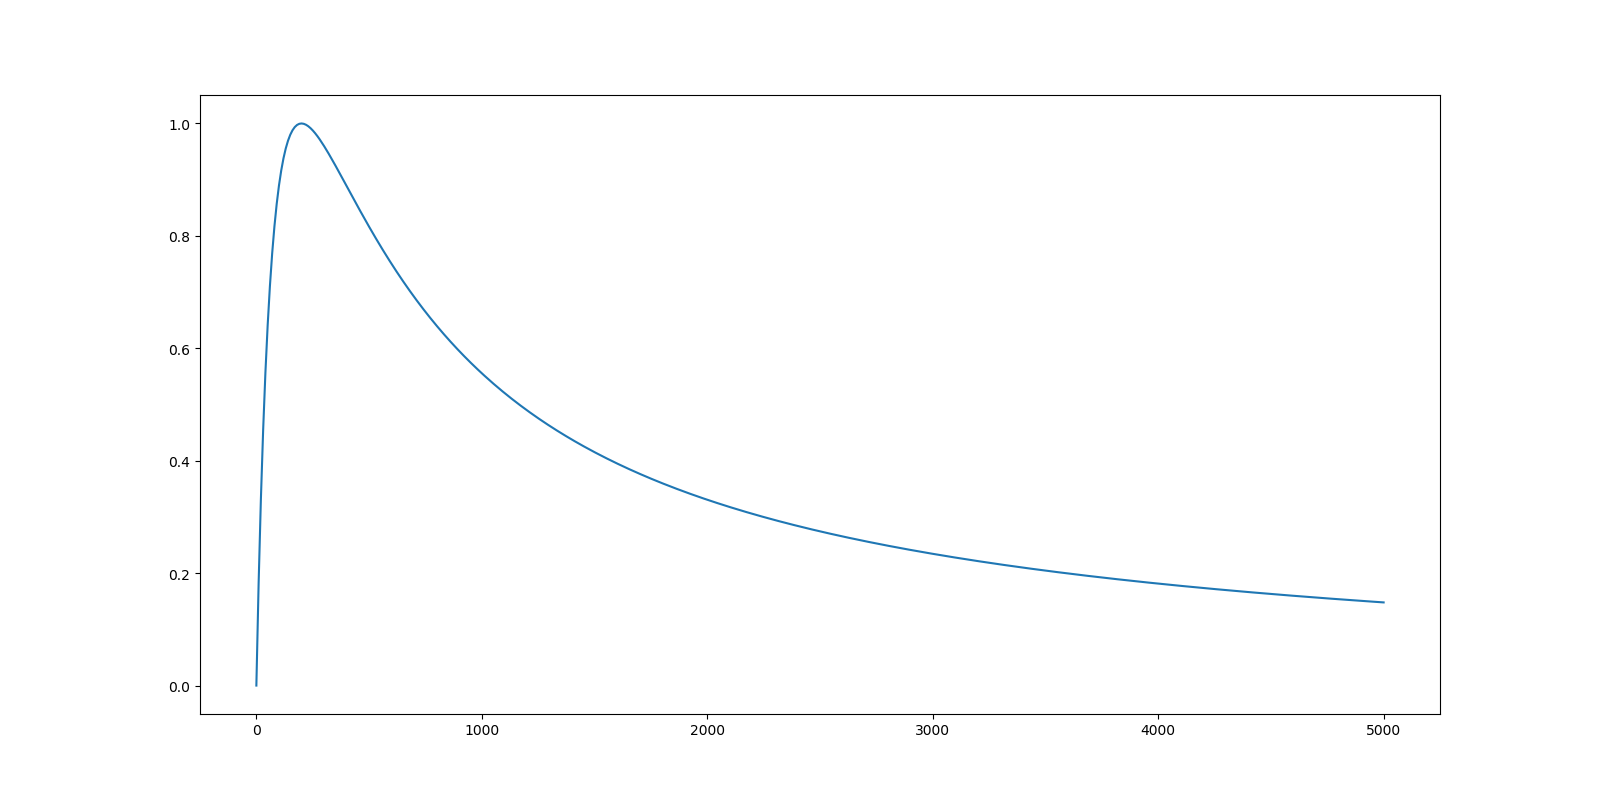
\includegraphics[width=\textwidth]{exercise1b.png}
The figure shows the behaviour of $r$ for fixed $m_\chi = 100 [random mass unit]$. One can see that for a target mass of zero r is zero as well. Going towards $m_\chi$ r rises fast to 1 ($m_\chi \approx m_T$). For $m_\chi << m_T$ r decreases towards zero again, but now the decrease is much weaker than the increase for $m_T << m_\chi$.

\paragraph{c)}
First case: $m_\chi = 10 \frac{GeV}{c^2} \rightarrow E_{kin} = 5\ MeV$.
\begin{align*}
&E_{r, e} = 1.022\ keV \\
&E_{r, p} = 1.568\ MeV \\
&E_{r, Si} = 3.992\ MeV \\
&E_{r, Xe} = 1.390\ MeV 
\end{align*} 
Where for the mass of Si 14 proton and 14 neutron masses were added and for Xe 54 proton and 77 neutron masses.\\
Second case: $m_\chi = 100 \frac{GeV}{c^2} \rightarrow E_{kin} = 50\ MeV$.
\begin{align*}
&E_{r, e} = 1.022\ keV \\
&E_{r, p} = 1.841\ MeV \\
&E_{r, Si} = 32.969\ MeV \\
&E_{r, Xe} = 49.467\ MeV 
\end{align*} 

\paragraph{d)}
Now one gets a scalar product at the point in a) where we have $2p_1p_3$ leading to $2p_1p_3 cos \theta$. Following the same calculation one gets the additional factor $(1 - cos \theta) / 2$, which is equal to one and maximal for $\theta = 180^\circ$, confirming the assumption of maximal momentum transfer for that angle in a).
\end{document}